\documentclass{standalone}
\usepackage{tikz, pgfplots, amssymb, amsmath, amsfonts}
\pgfplotsset{compat=1.18}
\newcommand{\vect}[1]{\boldsymbol{\mathbf{#1}}}
\pgfplotsset{ticks=none,axis x line=bottom,axis y line=left,enlargelimits=false}
\begin{document}
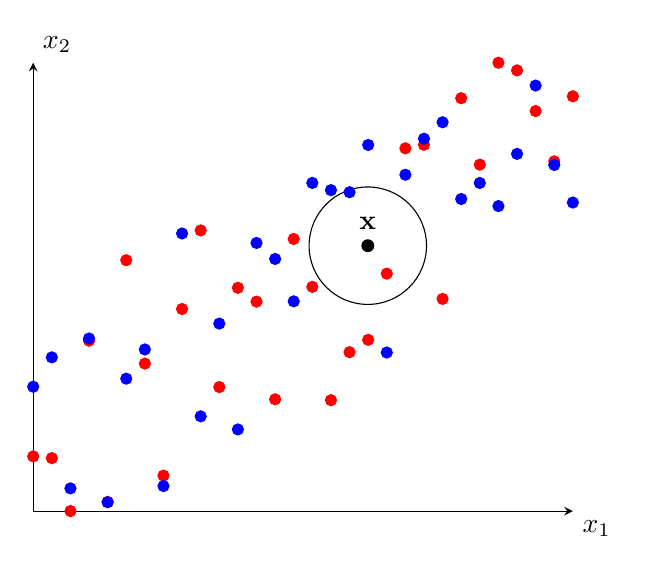
\begin{tikzpicture}
\begin{axis}[
    xlabel=$x_1$,ylabel=$x_2$,
    xlabel style={at={(ticklabel* cs:1)},anchor=north west},
    ylabel style={at={(ticklabel* cs:1)},anchor=south west},
    ylabel style={rotate=-90},]
    \addplot[only marks,samples=30, color=red]{0.75*x+3.5*rand};
    \addplot[only marks,samples=30, color=blue]{0.75*x+3.5*rand};
    \draw (1.2,1.2)node[draw, fill=black, circle, inner sep=1.5pt, label={$\vect{x}$}]{}node[circle, draw, inner sep=15pt]{};
\end{axis}
\end{tikzpicture}
\end{document}